
\chapter{Modelo Físico}

O problema foi definido como um canal plano, com apenas uma dimensão finita no eixo $ y $. Duas paredes de fronteira foram definidas como placas infinitas em condição de não deslizamento e em regime de fluxo térmico constante. O eixo $ z $ foi proposto como similar tanto na velocidade quanto na temperatura, resultando em um domínio plano (Fig.\ref{figure.1}). \\
A corrente foi considerado incompressível e o fluido foi considerado newtoniano. O fluido flui na direção do eixo $ x $. Os números da Reynolds variam de $ 4560 $ a $ 41441 $, resultando em um regime turbulento.

\begin{figure}[h!]
	\centering
	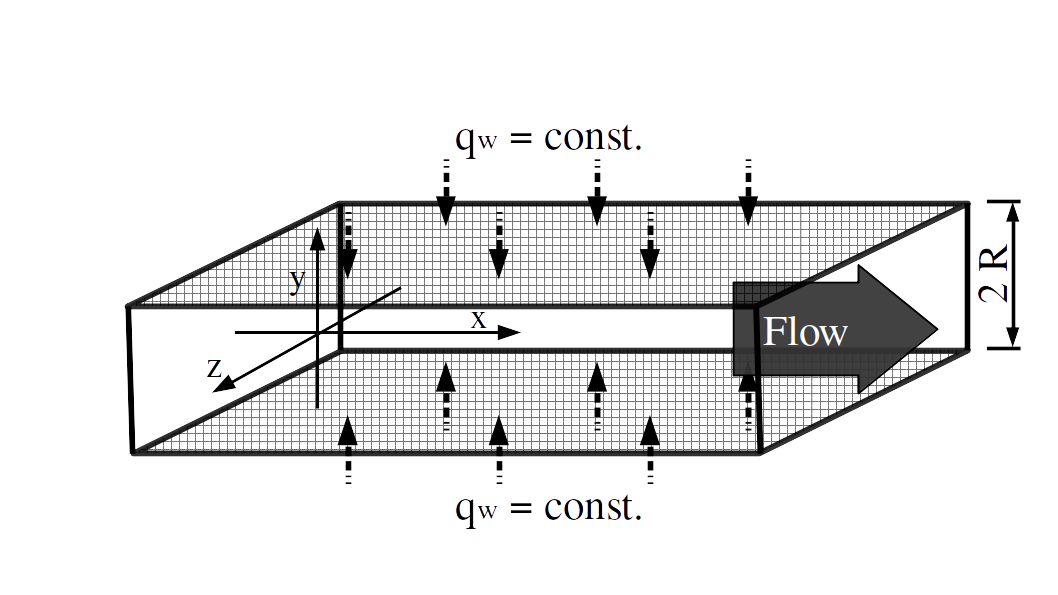
\includegraphics[angle=0, trim={0mm 10mm 0mm 20mm} , clip , scale=0.50]{fotos_formatacao_final/canal1}
	\caption{Definição geométrica do sistema e fronteiras.}
	\label{figure.1}
\end{figure}

A formulação matemática básica para o problema foram as equações de Navier-Stokes e da continuidade que são apresentadas no livro de Cengel \cite{Cengel}, e a equação de transporte de energia térmica, como apresentada no Incropera \cite{Incropera} de Freank. Estas foram as hipóteses feitas ao problema proposto, que serão consideradas no modelo matemático diferencial a seguir.



\chapter{Modelo Matemático Diferencial}
A equação média da continuidade (Eq.\ref{mass}), a equação média de Navier-Stokes em um eixo cartesiano (Eq.\ref{dynamics}) e a equação média do balanço de energia (Eq.\ref{energy permanent}) são apresentadas a diante: 


\begin{equation}\label{mass}
\frac{\partial \overline{u}}{\partial x} = 0.
\end{equation}

\begin{equation}\label{dynamics}
\frac{\partial \overline{u}\overline{v}}{\partial y} = 
- \frac{1}{\rho} \frac{\partial \overline{p}}{\partial x} + \frac{\partial}{\partial y}\left(\nu \frac{\partial \overline{u}}{\partial y} - \overline{u^\prime v^\prime}\right).
\end{equation}


\begin{equation}\label{energy permanent}
\frac{\partial{}}{\partial{x}} \left(\overline{T^\prime u^\prime}\right) + \frac{\partial{}}{\partial{x}}\left(\overline{u}.\overline{T}\right)     + 
\frac{\partial{}}{\partial{y}} \left(\overline{T^\prime v^\prime}\right) + \frac{\partial{}}{\partial{y}}\left(\overline{v}.\overline{T}\right) 
=
{\frac{\partial{}}{\partial{x}}} \left(\alpha {\frac{\partial{\overline{T}}}{\partial{x}}} \right) +
{\frac{\partial{}}{\partial{y}}} \left(\alpha {\frac{\partial{\overline{T}}}{\partial{y}}} \right). 
\end{equation}


A independência quanto ao tempo e o tratamento em valores médios tornam esta uma metodologia de Reynolds Averaged Navier Stokes (RANS).

\section{O regime permanente da temperatura}

O campo de velocidade é completamente desenvolvido no canal, para valores médios (fig.\ref{figure.3}), mas este não é o caso do campo de temperatura, pois um fluxo térmico constante é imposto sobre as paredes.
Mesmo considerando os valores médios, o campo de temperatura de uma correnteza em um canal turbulento não converge naturalmente para um estado permanente unidimensional (fig.\ref{figure.2}). O campo de velocidade está completamente desenvolvido, mas este não é o caso do campo de temperatura, pois um fluxo térmico constante é imposto sobre as paredes.

Em um esforço para simplificar a solução, a configuração térmica foi estudada com uma equação de balanço de energia térmica (\ref{c_h_e}).
\begin{figure}[h!]
	\centering
	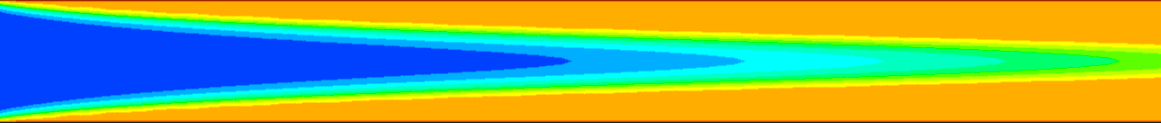
\includegraphics[angle=0, scale=0.40]{fotos_formatacao_final/temperatura}
	\caption{Campo de temperatura em regime estatístico permanente sobre um canal.}
	\label{figure.2}
\end{figure}
\begin{figure}[h!]
	\centering
	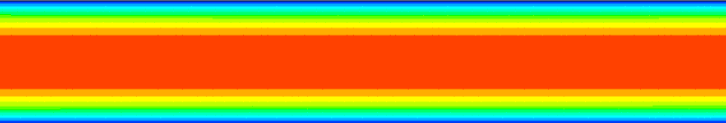
\includegraphics[angle=0, height=1.4cm , width=12.3cm]{fotos_formatacao_final/velocidade}
	\caption{campo de velocidade em regime completamente desenvolvido ao longo de um canal.}
	\label{figure.3}
\end{figure}


\begin{equation}\label{c_h_e}
q_{conv.} = \dot{m} C_p \Delta T_m,
\end{equation}
\begin{equation}
2q_w b \Delta x = \dot{m} C_p \Delta T_m,
\end{equation}\\



sendo $b$ a profundidade do canal e $T_m$ a temperatura média em uma secção transversal. Então, substituindo $ \dot{m} = u_m 2R b \rho $, e assumindo $ \Delta T_m = \frac{\partial{\left(\overline{T}_m\right)}}{\partial{x}} \Delta x $:
\begin{equation}
2q_w b \Delta x = u_m 2R b \rho  C_p \frac{\partial{\left(\overline{T}_m\right)}}{\partial{x}} \Delta x.
\end{equation}     
\begin{equation}
q_w = u_m R \rho  C_p \frac{\partial{\left(\overline{T}_m\right)}}{\partial{x}} .
\end{equation} 
\begin{equation}\label{c_h_ee}
\frac{\partial{\left(\overline{T}_m\right)}}{\partial{x}} = \frac{q_w}{u_m  R \rho  C_p } .
\end{equation} 

Como todos os termos no lado direito são constantes, a temperatura média teve que variar linearmente na direção do fluxo.
Para entender melhor a temperatura da parede com esse perfil de energia, foi realizado um estudo convectivo do fluxo térmico, que pode ser expresso matematicamente por:
\begin{equation}
q_w = h A \left( T_w(x) - \overline{T}_m(x)\right).
\end{equation}
É válido observar que $h$ é constante visto que este é um escoamento completamente desenvolvido. Assim, é possível escrever:
%\begin{equation}
%T_w(x) - \overline{T}_m(x) = \frac{q_w}{hA}.
%\end{equation}
%\begin{equation}
%\frac{d T_w(x)}{d x} - \frac{d \overline{T}_m(x)}{d x} = \frac{d \frac{q_w}{hA}}{dx}.
%\end{equation}
\begin{equation}
\frac{d T_w(x)}{d x} = \frac{d \overline{T}_m(x)}{d x} = Cte.
\end{equation}	

Com a temperatura nas paredes e o gradiente médio de temperatura definido como linear por essas determinações matemáticas, foi possível estender esse gradiente para todo o domínio considerando as condições de contorno e a simetria do sistema. Assim, um gradiente de temperatura constante foi imposto nas paredes aquecidas, criando uma condição de contorno de fluxo térmico constante, resultando em todo o campo de temperatura para variar linearmente no eixo $x$. A temperatura foi decomposta então na forma $ T^\ast(y) = T(x,y) - T_w(x) $ onde $T_w(x)$ é a temperatura nas paredes, resultando em uma simetria no sentido da corrente, diminuindo o problema a um unidimensional representativo para a variável $T^\ast(y)$. Assim, a expressão foi substituída em (\ref{energy permanent}):



\begin{equation}
\begin{split}
\frac{\partial{}}{\partial{x}} \left(\overline{(T^\ast + T_w)^\prime} \overline{ u^\prime}\right) + \frac{\partial{}}{\partial{x}}\left(\overline{(T^\ast + T_w)} \overline{u}\right)+ 
\frac{\partial{}}{\partial{y}} \left(\overline{(T^\ast + T_w)^\prime} \overline{ v^\prime}\right) + \frac{\partial{}}{\partial{y}}\left(\overline{(T^\ast + T_w)} \overline{v}\right) = \\
{\frac{\partial{}}{\partial{x}}} \left(\alpha {\frac{\partial{\overline{(T^\ast + T_w)}}}{\partial{x}}} \right) +
{\frac{\partial{}}{\partial{y}}} \left(\alpha {\frac{\partial{\overline{(T^\ast + T_w)}}}{\partial{y}}} \right) 
\end{split}
\end{equation}

Então a expressão poderia ser mais desenvolvida algebricamente considerando toda a velocidade média em $y$ e $z$ nulas:

\begin{equation}\label{equation_var}
{\frac{\partial{}}{\partial{y}}} \left(\alpha {\frac{\partial{\overline{T^\ast}}}{\partial{y}}}   
- \left(\overline{ T^{\ast\prime} v^\prime}\right) \right)
= 
\overline{u}\frac{\partial{}}{\partial{x}}\left(\overline{T_w}\right)  
\end{equation}



\section{A hipótese de Boussinesq}

Agora, em uma expressão simplificada unidimensional, o modelo requer um modelo de fechamento para o fluxo turbulento de energia térmica. Assim, a hipótese de Boussinesq foi usada. O termo $\overline{T^{\ast\prime}  v^\prime}$ pode ser modelado com:
\begin{equation}\label{bou}
-\left(\overline{ T^{\ast\prime}  v^\prime}\right) = 
\alpha_t \frac{\partial{\overline{T^\ast}}}{\partial{y}}.
\end{equation}
Assim, a seguinte equação pode ser obtida substituindo na equação principal (\ref{equation_var}):
\\
\begin{equation}
{\frac{\partial{}}{\partial{y}}} \left[(\alpha + \alpha_t)  \frac{\partial \overline{T^\ast}}{\partial y} \right]
= 
\overline{u}\frac{\partial{}}{\partial{x}}\left(\overline{T_w}\right) . 
\end{equation}

\section{O modelo de comprimento de mistura de Prandtl} 

O termo da difusão térmica turbulenta, $\alpha_t$, precisava ser modelado. O conceito clássico do número de Prandtl turbulento é usado no presente trabalho:
\begin{equation}
Pr_t = \frac{\nu_t}{\alpha_t}.
\end{equation} 
O termo $ \nu_t $ precisa ser modelado. O valor clássico do número de Prandtl turbulento $ Pr_t = 0.71 $ foi utilizado.
Com o modelo do comprimento de mistura de Prandtl, é postulado que:
\begin{equation}
\nu_t = {l^2_m} \left| \frac{\partial \overline{u}}{\partial y} \right|.
\end{equation}
O comprimento de mistura introduz um módulo no modelo diferencial, bem como o parâmetro do número de Prandtl turbulento:
\\
\begin{equation}
{\frac{\partial{}}{\partial{y}}} \left( \left( \alpha   
+ \frac{\nu_t}{Pr_t} \right) \frac{\partial \overline{T^\ast}}{\partial y} \right)
= 
\overline{u}\frac{\partial{}}{\partial{x}}\left(\overline{T_w}\right)  .
\end{equation}
\begin{equation}\label{equationquasela}
{\frac{\partial{}}{\partial{y}}} \left( \left( \alpha   
+ \frac{{l^2_m} \left| \frac{\partial \overline{u}}{\partial y} \right|}{Pr_t} \right) \frac{\partial \overline{T^\ast}}{\partial y} \right)
= 
\overline{u}\frac{\partial{}}{\partial{x}}\left(\overline{T_w}\right)  .
\end{equation}
\\

É possível perceber, ao analisar a dinâmica do fluxo, que para valores positivos de $ y $, ver figura \ref{figure.1}, a primeira derivada da velocidade será sempre negativa, pois temos uma velocidade que diminui com o aumento de $ y $. Isso implica em:\\
\begin{equation}
{\frac{\partial{}}{\partial{y}}} \left( \left( \alpha   
- \frac{{l^2_m}}{Pr_t}\frac{\partial \overline{u}}{\partial y} \right) \frac{\partial \overline{T^\ast}}{\partial y} \right)
= 
\overline{u}\frac{\partial{}}{\partial{x}}\left(\overline{T_w}\right)  .
\end{equation}



\section{O comprimento de mistura}

O comprimento de mistura $ l_m $ precisa ser modelado. Pode-se observar que os estudos experimentais de Nikuradse foram utilizados para modelar este parâmetro, conforme segue::
\begin{equation}
L\left(\frac{y}{R}\right) = \frac{l_m}{R} = 0.14 - 0.08 \left(\frac{y}{R}\right)^2 - 0.06\left(\frac{y}{R}\right)^4.
\end{equation}
Para completar ainda mais o modelo, Cebeci e Bradshaw adicionaram a função de amortecimento Van Driest:
\begin{equation}\label{eqution_mixturelength}
L\left(\frac{y}{R}\right)  = \frac{l_m}{R} = \left\{\frac{l_m}{R} = 0.14 - 0.08 \left(\frac{y}{R}\right)^2 - 0.06\left(\frac{y}{R}\right)^4\right\}\left\{  1 - e^{[(\tilde{y} - 1) \frac{Re_\tau}{A}]}\right\},
\end{equation}
Com $A = 26$ como a constante do Cebeci. Assim, teve-se o comprimento de mistura definido por:
\begin{equation}
lm = L R,
\end{equation}
$ L $ sendo uma função no eixo $ y $, dado pela equação (\ref{eqution_mixturelength}). Assim, a equação (\ref{equationquasela}) pode ser escrita como:
\begin{equation}\label{cebeciconstant}
{\frac{\partial{}}{\partial{y}}} \left( \left( \alpha   
- \frac{{L}^2 R ^2}{Pr_t}\frac{\partial \overline{u}}{\partial y} \right) \frac{\partial \overline{T^\ast}}{\partial y} \right)
= 
\overline{u}\frac{\partial{}\left(\overline{T_w}\right)  }{\partial{x}}.
\end{equation}
Para comparar o presente trabalho com modelos da literatura, esta equação foi adimensionalizada utilizando as coordenadas da parede. Foi considerado: $ \tilde{y} = \frac{y . Re_\tau}{R} $, $ \tilde{\overline{u}} = \frac{\overline{u}}{u_\tau} $ , $ \tilde{\overline{T}} = \frac{\overline{T}}{T_\tau} $ , $ \tilde{\overline{T^\ast}} = \frac{\overline{T^\ast}}{T_\tau} $ , $Re_\tau = \frac{u_\tau R}{\nu}$, $Pr_t = \frac{\nu_t}{\alpha_t}$, $Pr = \frac{\nu}{\alpha}$, $T_\tau = \frac{q_w}{\rho C_p u_\tau}$, $\frac{\partial{\left(T_m\right)}}{\partial{x}} = \frac{q_w}{u_m  R \rho  C_p } $ e $\frac{\partial \overline{p}}{\partial x} = - \frac{u_\tau^2 \rho}{R} $. Isso resultou em:
\\
\begin{equation}\label{equationultima}
{\frac{\partial{}}{\partial{\tilde{y}}}} \left( \left( \frac{Re_\tau}{Pr}   
- \frac{{L}^2 Re_\tau ^3}{Pr_t}\frac{\partial \tilde{\overline{u}}}{\partial \tilde{y}} \right) \frac{\partial \tilde{\overline{T^\ast}}}{\partial \tilde{y}} \right)
= 
\frac{\tilde{\overline{u}}}{\tilde{u_m}}.
\end{equation}
É importante notar que há a velocidade na equação (\ref{equationultima}), ou seja, para o desenvolvimento do problema térmico, é necessário o desenvolvimento do perfil de velocidades no canal. Para isso, um modelo RANS previamente feito (Antonialli and Silveira, 2015) foi usado, como segue:
\begin{equation}\label{finalequationvelocity}	
\frac{\partial \tilde{\overline{u}}}{\partial \tilde{y}} = - \frac{2 \tilde{y} \frac{1}{Re_\tau} }{ 1 + \sqrt{ 1 + 4 L ^2 Re_\tau ^2 \tilde{y}}}.
\end{equation}	
Desta forma, tivemos a primeira derivada da velocidade em uma forma exata.

